\title{Ecualización de señales en un enlace digital de comunicaciones}

\author{
    \IEEEauthorblockN{Rocío Parra}
    \IEEEauthorblockN{Lucero Guadalupe Fernandez}
    \IEEEauthorblockN{Instituto Tecnológico de Buenos Aires}
}

\maketitle

\begin{abstract}
\todo[inline]{hacer abstract ekis de}
\end{abstract}


\section{Introducción}
Se buscó ecualizar una señal en un enlace digital de comunicaciones. 
Los datos consistían en una secuencia de datos pseudoaleatoria 
codificada por Manchester, muestreada a una frecuencia de sampleo
 de $4kHz$ a razón de $250bps$. Ante estas características, cada bit consiste de 
 16 muestras según la codificación mencionada. El canal, en este caso, conocido, 
 modificaba la señal dependiendo del posicionamiento
 aleatorio de dos pares de polos conjugados.
La principal dificultad consistía entonces en la variabilidad del canal. En las 
siguientes figuras se puede notar el efecto de lo mencionado, siendo la 
señal en azul los bits enviados y en naranja lo recibido. \newline

\begin{figure}[h!]
    \centering
    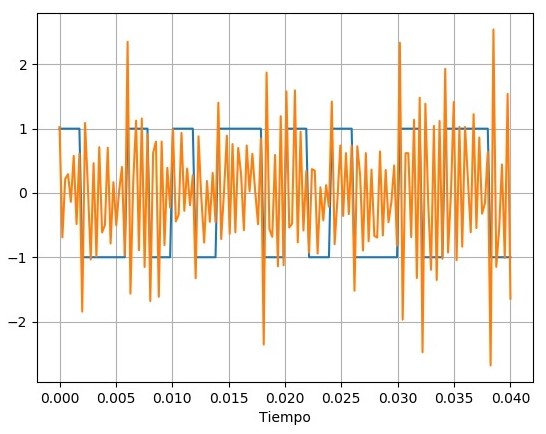
\includegraphics[scale=0.3]{imagenes/1.jpeg}
\end{figure}
\begin{figure}[h!]
    \centering
    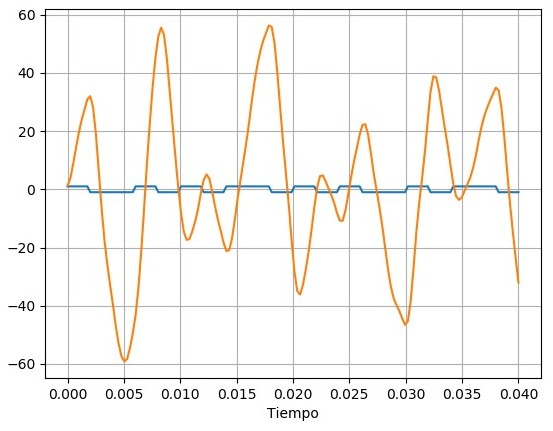
\includegraphics[scale=0.3]{imagenes/2.jpeg}
\end{figure}
\begin{figure}[h!]
    \centering
    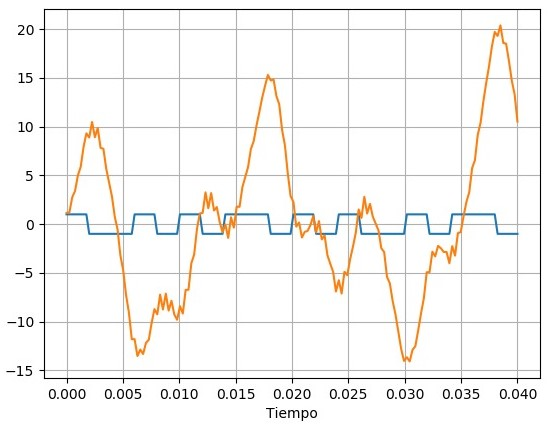
\includegraphics[scale=0.3]{imagenes/3.jpeg}
\end{figure}
\begin{figure}[h!]
    \centering
    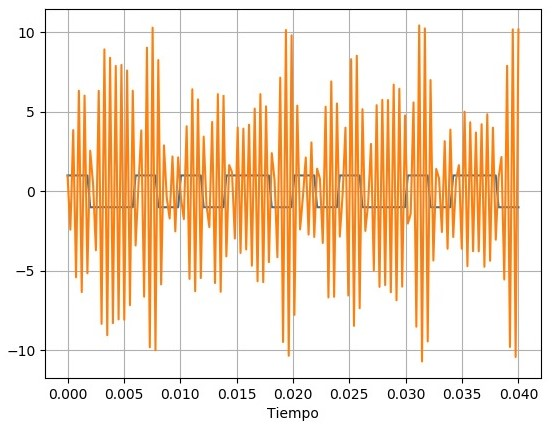
\includegraphics[scale=0.3]{imagenes/4.jpeg}
    \caption{Señales obtenidas en el receptor, al pasar por del canal.}
\end{figure}

El proyecto consiste en aplicar un algoritmo de filtrado adaptativo
 para recuperar la señal transmitida asumiendo que no se conoce la entrada, 
 lo que simularía enlace digital de comunicaciones, un esquema de lo mencionado
se puede ver en la siguiente figura.

\begin{figure}[h!]
    \centering
    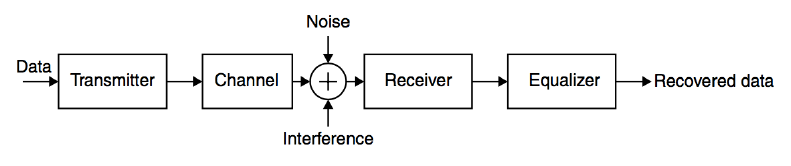
\includegraphics[scale=0.5]{imagenes/preblock.png}
    \caption{Esquema del enlace digital.}
\end{figure}

 \todo[inline]{hacer histograma de la energia random de las señales.}

